\documentclass[tikz, border=10pt]{standalone}
\usepackage{pgfplots}
\usepgfplotslibrary{fillbetween}
\pgfplotsset{compat=1.18}

\begin{document}
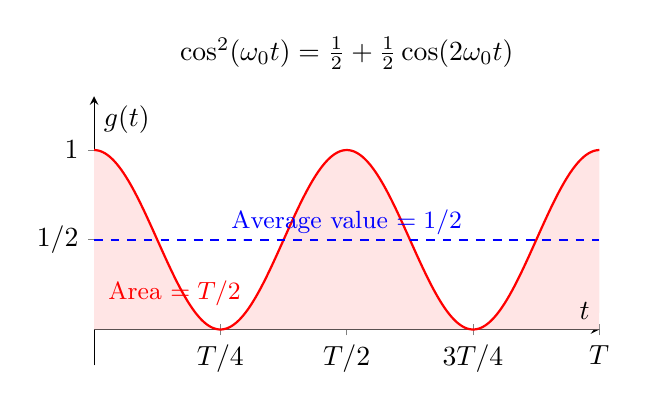
\begin{tikzpicture}
    \begin{axis}[
        width=8cm, height=5cm,
        axis lines=middle,
        xlabel={$t$}, ylabel={$g(t)$},
        xmin=0, xmax=2*pi,
        ymin=-0.2, ymax=1.3,
        xtick={0, 1.57, 3.14, 4.71, 6.28},
        xticklabels={0, $T/4$, $T/2$, $3T/4$, $T$},
        ytick={0, 0.5, 1},
        yticklabels={0, $1/2$, $1$},
        samples=400,
        domain=0:2*pi,
        title={$\cos^2(\omega_0 t) = \frac{1}{2} + \frac{1}{2}\cos(2\omega_0 t)$}
    ]
        % The squared function
        \addplot[name path=f, red, thick] {cos(deg(x))^2};
        \path[name path=axis] (axis cs:0,0) -- (axis cs:6.28,0);
        \addplot[red!10] fill between[of=f and axis];
        
        % The average line
        \addplot[blue, dashed, thick] {0.5};
        \node[blue, font=\small] at (axis cs:3.14, 0.6) {Average value $= 1/2$};
        
        % Integral markers
        \node[red, font=\small] at (axis cs:1, 0.2) {Area $= T/2$};
    \end{axis}
\end{tikzpicture}
\end{document}
